 \section{Our Approach}\label{back}
Figure~\ref{fig:figure1} introduces our holistic approach for understanding, repairing and verifying robustness issues in deep neural networks. 
Our proposed framework consists of four major tasks (\textbf{Tasks 1-4}) corresponding to the aforementioned four goals (\textbf{Goals  1-4}). 
Given a DNN model together with its training data and software configurations (e.g., hyperparameters and various training settings), \textbf{Task 1} aims to first study the training factors affecting the model's  robustness e.g., minor perturbations to the data and software configurations of the DNN, which cause to alter its outputs. We aim to capture the correlation between various robustness factors and actual model's behaviour for later mitigating and repairing robustness issues. Subsequently, our \textbf{Task 2} then aims to develop adversarial training to repair robustness issues by harness the imperfect data and various software configurations (studied in Task 1) through semi-supervised active-constrastive learning.

In order to boost efficiency of adversarial training, \textbf{Task 3} aims to develop a robustness-preserving model reduction approach to optimize the DNN structure by pruning the network parts which do not affect the robustness of the DNN. 
Our framework allows \textbf{Tasks 2 and 3} to be performed iteratively, thereby providing increasingly improved robustness and refined model structure for both training accuracy and efficiency.
In \textbf{Task 4}, we will investigate symbolic techniques to qualitatively measure the robustness property of the resulting model from Task 3. Finally, we will certify the robustness of a model \emph{w.r.t}  a lower robust bound (the perturbation distance under which a neural network is proved robust against any allowable perturbation) to  guarantee the model's robustness under an explicit condition. 

\begin{figure}[!t]
    \centering
    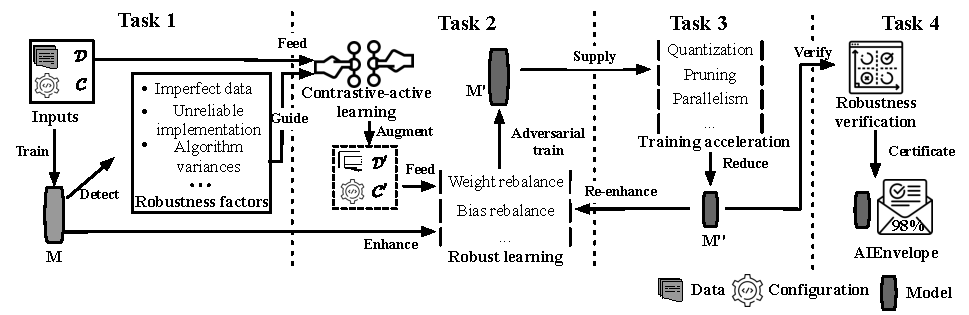
\includegraphics[width=\linewidth]{fig/approach-1.pdf}
    \caption{\mbox{AIEnvelope} framework}
    \label{fig:figure1}
\end{figure}
